% CH4114 --- Tutorial 00, Part 5: Lattice Structures
% Beamer deck, 16:9, compiled with pdflatex (TeX Live 2026)
% Author: Shuvam Banerji Seal
\documentclass[aspectratio=169]{beamer}

\usetheme{Madrid}
\usecolortheme{whale}
\setbeamertemplate{navigation symbols}{}

\usepackage[T1]{fontenc}
\usepackage{tikz}
\usetikzlibrary{arrows.meta, positioning}
\usepackage{booktabs}
\usepackage{listings}
\lstset{
  basicstyle=\ttfamily\footnotesize,
  breaklines=true,
  showstringspaces=false,
  columns=fullflexible,
  keepspaces=true,
}

\title[Lattice Structures]{Tutorial 00 --- Part 5\\[2pt] Lattice Structures: SCC, BCC, FCC}
\subtitle{2D and 3D plots + packing fractions}
\author[SBS]{Shuvam Banerji Seal}
\institute[CH4114]{CH4114 --- Molecular Simulation}
\date[Aug 2026]{14 August 2026}

\begin{document}

% ------------------------------------------------------------------ title
\begin{frame}[plain]
  \titlepage
  \centering{\scriptsize Course Instructor: Dr.\ Susmita Roy \quad$\cdot$\quad TA: Shuvam Banerji Seal}\par
  \vspace{0.1cm}
  \centering{\scriptsize Repository: \texttt{CH4114\_Molecular\_Simulation\_Tutorials}}
\end{frame}

% --------------------------------------------------------------- lattice
\begin{frame}{What is a crystal lattice?}
  \begin{columns}[T]
    \begin{column}{0.4\textwidth}
      \begin{center}
        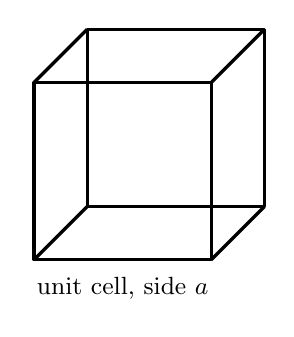
\begin{tikzpicture}[line join=round, scale=1.5]
          \draw[very thick] (0,0) rectangle (1.5,1.5);   % front face
          \draw[very thick] (0.45,0.45) rectangle (1.95,1.95);  % back face
          \draw[very thick] (0,0) -- (0.45,0.45);
          \draw[very thick] (1.5,0) -- (1.95,0.45);
          \draw[very thick] (1.5,1.5) -- (1.95,1.95);
          \draw[very thick] (0,1.5) -- (0.45,1.95);
          \node[below=0.1cm, font=\small] at (0.75,0) {unit cell, side $a$};
        \end{tikzpicture}
      \end{center}
    \end{column}
    \begin{column}{0.56\textwidth}
      \begin{itemize}
        \item A crystal is atoms in a \textbf{repeating pattern}.
        \item The smallest repeating unit is the \textbf{unit cell} --- a cube
              of side $a$ (the \emph{lattice constant}).
        \item Three classic cubic lattices: \textbf{SCC}, \textbf{BCC}, \textbf{FCC}.
      \end{itemize}
    \end{column}
  \end{columns}
\end{frame}

% ------------------------------------------------------------ the three
\begin{frame}{The three cubic lattices}
  \begin{table}
    \small
    \begin{tabular}{@{}llll@{}}
      \toprule
      Lattice & Atoms per cell & Radius $r$ & Coordination \\
      \midrule
      SCC & 1 (8 corners $\times \frac{1}{8}$) & $a/2$ & 6 \\
      BCC & 2 ($\frac{1}{8}$ corners $+$ 1 center) & $a\sqrt{3}/4$ & 8 \\
      FCC & 4 ($\frac{1}{8}$ corners $+$ 6 faces $\times \frac{1}{2}$) & $a\sqrt{2}/4$ & 12 \\
      \bottomrule
    \end{tabular}
  \end{table}
  \vspace{0.3cm}
  \begin{itemize}
    \item Neighboring atoms just \textbf{touch}:
    \item SCC along the \emph{edge} ($2r=a$), BCC along the \emph{body
          diagonal} ($4r=a\sqrt{3}$), FCC along the \emph{face diagonal} ($4r=a\sqrt{2}$).
  \end{itemize}
\end{frame}

% -------------------------------------------------------------- 2d views
\begin{frame}[fragile]{2D top views of the unit cells}
  \begin{center}
    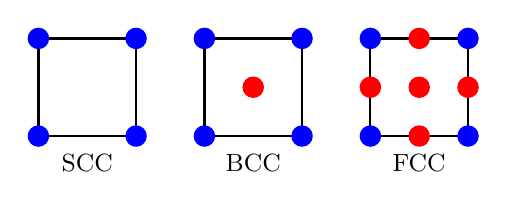
\begin{tikzpicture}[scale=0.62, every node/.style={font=\small}]
      % SCC
      \draw[thick] (0,0) rectangle (2,2);
      \foreach \x/\y in {0/0, 2/0, 2/2, 0/2} \fill[fill=blue] (\x,\y) circle (0.22);
      \node at (1,-0.55) {SCC};
      % BCC
      \begin{scope}[xshift=3.4cm]
        \draw[thick] (0,0) rectangle (2,2);
        \foreach \x/\y in {0/0, 2/0, 2/2, 0/2} \fill[fill=blue] (\x,\y) circle (0.22);
        \fill[fill=red] (1,1) circle (0.22);
        \node at (1,-0.55) {BCC};
      \end{scope}
      % FCC
      \begin{scope}[xshift=6.8cm]
        \draw[thick] (0,0) rectangle (2,2);
        \foreach \x/\y in {0/0, 2/0, 2/2, 0/2} \fill[fill=blue] (\x,\y) circle (0.22);
        \foreach \x/\y in {1/0, 1/2, 0/1, 2/1, 1/1} \fill[fill=red] (\x,\y) circle (0.22);
        \node at (1,-0.55) {FCC};
      \end{scope}
    \end{tikzpicture}
  \end{center}
  \vspace{0.2cm}
  \begin{itemize}
    \item \textcolor{blue}{blue} = corners, \textcolor{red}{red} = body/face centers.
    \item FCC seen from above: edge midpoints + the top-face center.
  \end{itemize}
\end{frame}

% ------------------------------------------------------------ 2d packing
\begin{frame}[fragile]{Packing fraction in 2D}
  \begin{columns}[T]
    \begin{column}{0.4\textwidth}
      \begin{center}
        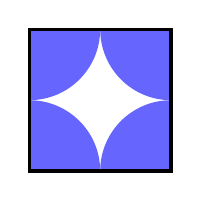
\begin{tikzpicture}[scale=0.9]
          \begin{scope}
            \clip (0,0) rectangle (2,2);
            \foreach \x/\y in {0/0, 2/0, 2/2, 0/2} \fill[fill=blue!60] (\x,\y) circle (1);
          \end{scope}
          \draw[very thick] (0,0) rectangle (2,2);
        \end{tikzpicture}
      \end{center}
    \end{column}
    \begin{column}{0.56\textwidth}
      \begin{itemize}
        \item Packing fraction = area of atoms $\div$ total area.
        \item \textbf{Square lattice}: cell side $2r$, one circle per cell
              \[ \frac{\pi r^2}{(2r)^2} = \frac{\pi}{4} \approx 0.7854 \]
        \item \textbf{Hexagonal lattice}: the densest 2D packing
              \[ \frac{\pi r^2}{2\sqrt{3}\,r^2} = \frac{\pi}{2\sqrt{3}} \approx 0.9069 \]
      \end{itemize}
    \end{column}
  \end{columns}
\end{frame}

% -------------------------------------------------------------- 3d cells
\begin{frame}[fragile]{3D unit cells with Matplotlib}
  \begin{columns}[T]
    \begin{column}{0.5\textwidth}
      \begin{lstlisting}[basicstyle=\ttfamily\scriptsize]
def unit_cell_atoms(kind):
    corners = [(x, y, z)
      for x in (0, a) for y in (0, a)
      for z in (0, a)]
    if kind == "SCC":
        return np.array(corners)
    if kind == "BCC":
        return np.array(corners
          + [(a/2, a/2, a/2)])
    if kind == "FCC":
        faces = [(0, a/2, a/2), (a, a/2, a/2),
                 (a/2, 0, a/2), (a/2, a, a/2),
                 (a/2, a/2, 0), (a/2, a/2, a)]
        return np.array(corners + faces)
      \end{lstlisting}
    \end{column}
    \begin{column}{0.46\textwidth}
      \begin{itemize}
        \item Scatter the atoms inside a cube.
        \item Draw the 12 cube edges so the cell is visible.
        \item One 3D subplot per lattice: \texttt{subplot(1,3,i, projection="3d")}.
      \end{itemize}
      \vspace{0.2cm}
      \begin{alertblock}{ Drag to rotate}
        The 3D plot is interactive --- rotate, zoom, inspect.
      \end{alertblock}
    \end{column}
  \end{columns}
\end{frame}

% ------------------------------------------------------------ 3d packing
\begin{frame}{Packing fraction in 3D}
  \begin{table}
    \small
    \begin{tabular}{@{}llll@{}}
      \toprule
      Lattice & Atoms & Radius & Packing fraction \\
      \midrule
      SCC & 1 & $a/2$ & $\pi/6 \approx 0.5236$ \\
      BCC & 2 & $a\sqrt{3}/4$ & $\sqrt{3}\,\pi/8 \approx 0.6802$ \\
      FCC & 4 & $a\sqrt{2}/4$ & $\pi/(3\sqrt{2}) \approx 0.7405$ \\
      \bottomrule
    \end{tabular}
  \end{table}
  \vspace{0.3cm}
  \begin{block}{Formula}
    \[
      \text{packing fraction} =
      \frac{\text{atoms per cell} \times \frac{4}{3}\pi r^3}{a^3}
    \]
  \end{block}
  \begin{itemize}
    \item \textbf{FCC is the most efficient} (74\%) --- why copper, gold,
          aluminum crystallize in FCC.
  \end{itemize}
\end{frame}

% ------------------------------------------------------------ monte carlo
\begin{frame}[fragile]{Verify with Monte Carlo (random points)}
  \begin{columns}[T]
    \begin{column}{0.4\textwidth}
      \begin{center}
        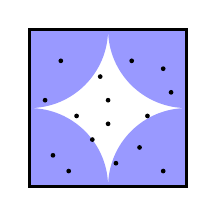
\begin{tikzpicture}[scale=1.0]
          \begin{scope}
            \clip (0,0) rectangle (2,2);
            \foreach \x/\y in {0/0, 2/0, 2/2, 0/2} \fill[fill=blue!40] (\x,\y) circle (1);
          \end{scope}
          \draw[very thick] (0,0) rectangle (2,2);
          \foreach \x/\y in {0.3/0.4, 0.5/0.2, 0.8/0.6, 1.1/0.3, 1.4/0.5, 1.7/0.2,
                             0.2/1.1, 0.6/0.9, 1.0/0.8, 1.5/0.9, 1.8/1.2,
                             0.4/1.6, 0.9/1.4, 1.3/1.6, 1.7/1.5, 1.0/1.1}
            \fill[fill=black] (\x,\y) circle (0.03);
        \end{tikzpicture}
      \end{center}
    \end{column}
    \begin{column}{0.56\textwidth}
      \begin{itemize}
        \item Throw $N$ random points into the cube with \texttt{np.random}.
        \item Count how many fall \textbf{inside} an atom.
        \item Fraction inside $\approx$ packing fraction.
      \end{itemize}
      \vspace{0.2cm}
      \begin{lstlisting}[basicstyle=\ttfamily\scriptsize]
np.random.seed(42)
pts = np.random.rand(N, 3) * a
frac = inside_any(pts, atoms, r).mean()
print(frac)   # FCC -> ~0.7405
      \end{lstlisting}
      \begin{itemize}
        \item The simulation agrees with the math!
      \end{itemize}
    \end{column}
  \end{columns}
\end{frame}

% ------------------------------------------------------------- interactive
\begin{frame}[fragile]{Interactive 3D rotation}
  \begin{block}{In a script}
    \texttt{plt.show()} opens a window --- drag to rotate, scroll to zoom.
  \end{block}
  \begin{block}{In a Jupyter notebook}
    \begin{lstlisting}
%matplotlib widget      # interactive figures (needs: uv add --dev ipympl)
    \end{lstlisting}
  \end{block}
  \begin{itemize}
    \item \textbf{Drag} left button $\rightarrow$ rotate the lattice.
    \item \textbf{Right-drag} $\rightarrow$ zoom.
    \item \textbf{Scroll} $\rightarrow$ zoom in/out.
    \item Inspect the atom positions from every angle.
  \end{itemize}
\end{frame}

% --------------------------------------------------------------- summary
\begin{frame}[fragile]{Scripts, notebooks, and check yourself}
  \begin{block}{Run the companion code}
    \begin{lstlisting}
uv run python examples/lattice_structures/lattice_2d.py
uv run python examples/lattice_structures/lattice_3d.py
uv run python examples/lattice_structures/packing_fraction.py
    \end{lstlisting}
  \end{block}
  \begin{block}{Check yourself}
    \begin{enumerate}
      \item How many atoms does an FCC unit cell contain? Why 4, not 14?
      \item Why is the BCC atom radius $a\sqrt{3}/4$ and not $a/2$?
      \item Which lattice has the highest packing fraction?
      \item What is the 2D packing fraction of a square lattice?
      \item Why set \texttt{np.random.seed(...)} before the Monte Carlo check?
    \end{enumerate}
  \end{block}
\end{frame}

\end{document}